\section{Perturbed bows}
\label{sec:perturbed-bows}

\begin{figure}
  \centering
  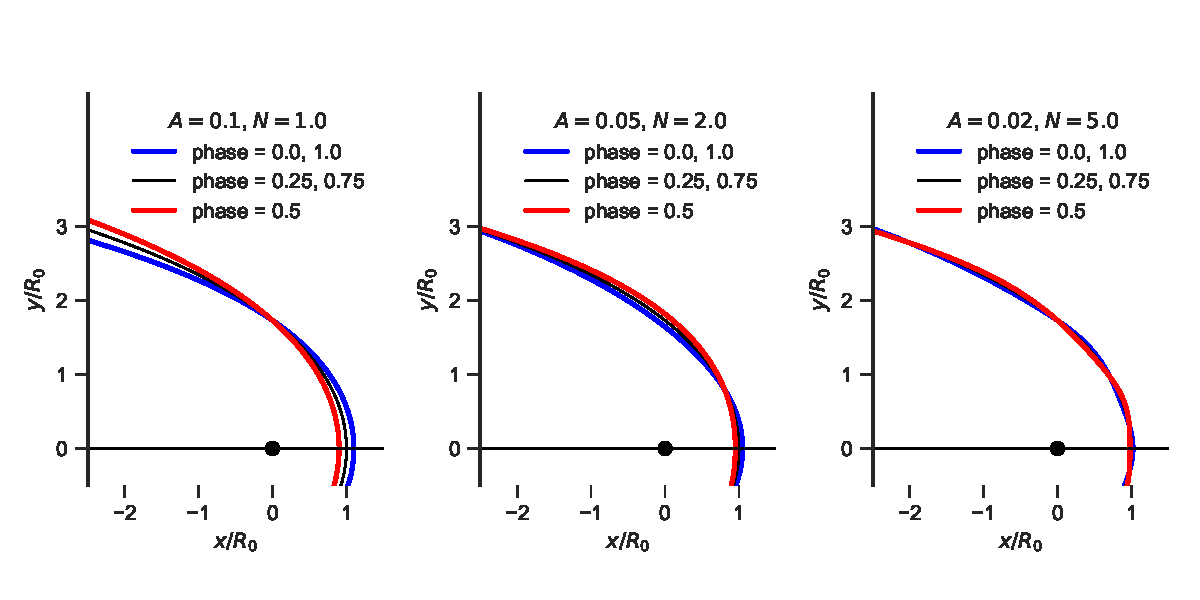
\includegraphics[width=\linewidth]{figs/compare_xyprime_wave-wilkinoid}
  \caption{Small-amplitude standing wave perturbations to bow shapes.}
  \label{fig:perturb-shapes}
\end{figure}

\begin{figure}
  \centering
  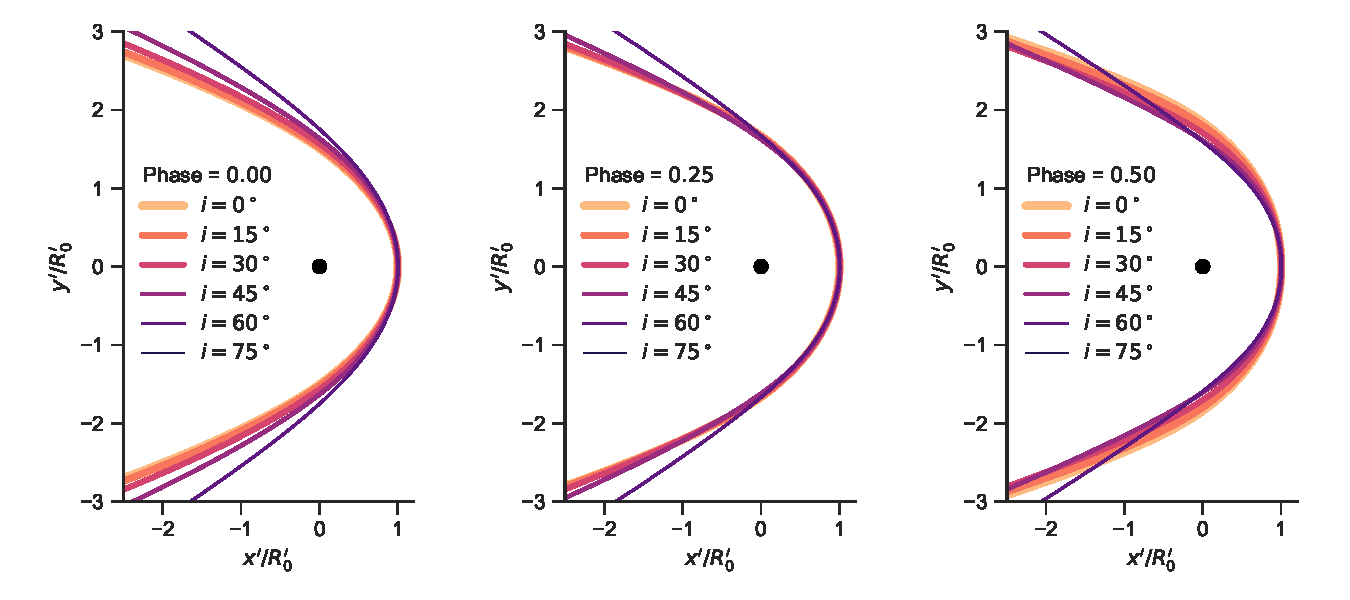
\includegraphics[width=\linewidth]
  {figs/wave_xyprime-A005-N20-ancantoid-xi080-beta000500}
  \caption{Plane-of-sky projections of perturbed bow shapes}
  \label{fig:perturb-xy-prime}
\end{figure}


\begin{figure}
  \centering
  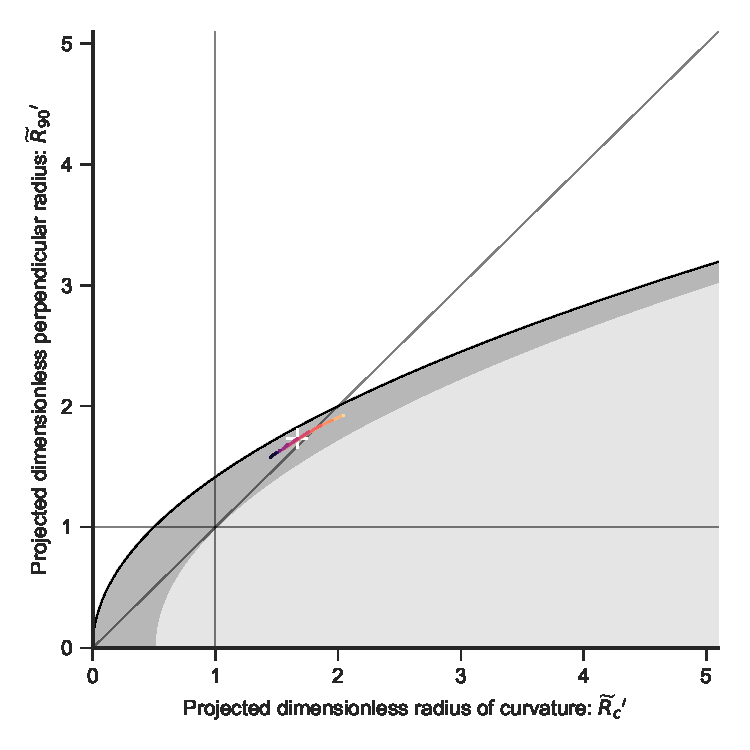
\includegraphics[width=\linewidth]
  {figs/wilkinoid-R90-vs-Rc-wave-A010-N10}
  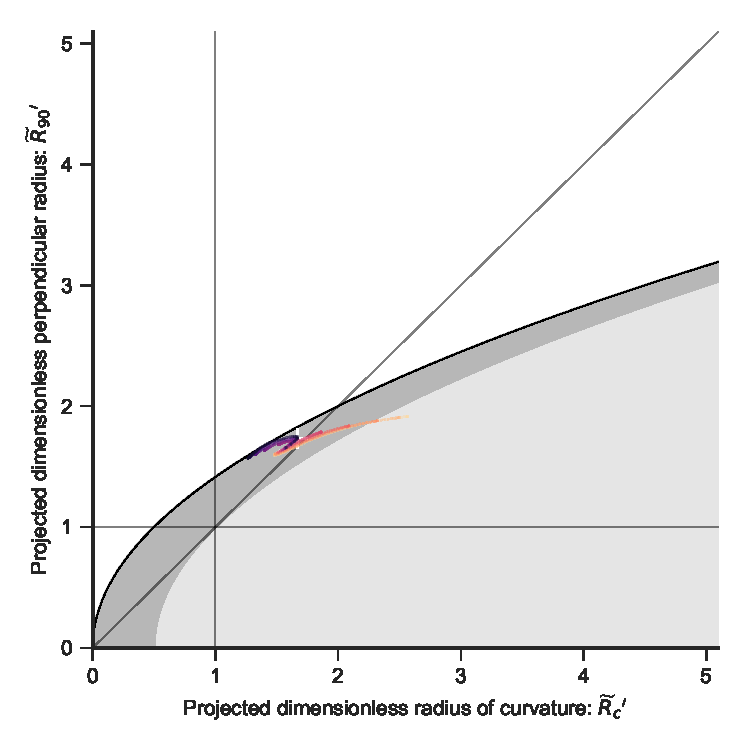
\includegraphics[width=\linewidth]
  {figs/wilkinoid-R90-vs-Rc-wave-A005-N20}
  \caption{Diagnostic diagram for perturbed shapes}
  \label{fig:perturb-Rc-R90}
\end{figure}


%%% Local Variables:
%%% mode: latex
%%% TeX-master: "quadrics-bowshock"
%%% End:
